
\documentclass[tikz,border=0pt]{standalone}
\usepackage{tikz}
\begin{document}
\tikzset{every picture/.style={line width=0.75pt}}
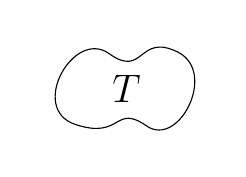
\begin{tikzpicture}[x=0.75pt,y=0.75pt,yscale=-1,xscale=1]

\draw   (90.73,72.5) .. controls (109.91,82.03) and (91.3,118.97) .. (75.61,108.04)
.. controls (59.92,97.12) and (63.98,114.87) .. (41.32,107.36)
.. controls (18.65,99.85) and (40.59,61) .. (57.59,73.22)
.. controls (74.6,85.43) and (71.54,62.97) .. (90.73,72.5) -- cycle ;

\node at (66,90) {\Large $T$};

\end{tikzpicture}
\end{document}
